\documentclass[../../main.tex]{subfiles}

\begin{document}

\begin{figure}[ht]
\centering
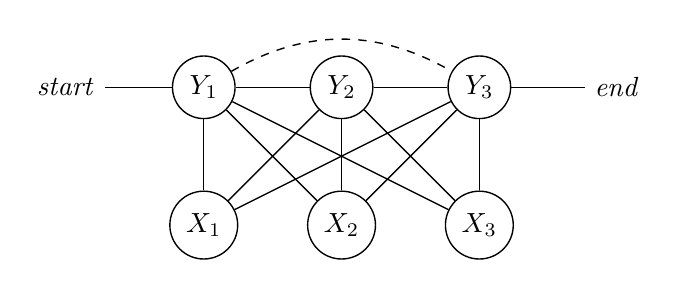
\begin{tikzpicture} [line width = 0.5pt, node distance = 1.75cm]

\node (start) {\textit{start}};
\node [circle, draw] (y1) [right of = start] {$Y_1$};
\node [circle, draw] (y2) [right of = y1] {$Y_2$};
\node [circle, draw] (y3) [right of = y2] {$Y_3$};
\node (end) [right of = y3] {\textit{end}};

\path (start) edge (y1);
\path (y1) edge (y2);
\path (y2) edge (y3);
\path (y3) edge (end);

\node [circle, draw] (x1) [below of = y1] {$X_1$};
\node [circle, draw] (x2) [below of = y2] {$X_2$};
\node [circle, draw] (x3) [below of = y3] {$X_3$};

\path (y1) edge (x1);
\path (y2) edge (x2);
\path (y3) edge (x3);

\path (y1) edge [dashed, bend left] (y3);

\path (y1) edge (x2);
\path (y1) edge (x3);

\path (y2) edge (x1);
\path (y2) edge (x3);

\path (y3) edge (x1);
\path (y3) edge (x2);

\end{tikzpicture}
\caption{A conditional random field applied to the part-of-speech tagging problem. The dashed arc between $Y_1$ and $Y_3$ would be prohibited in a linear-chain model.}
\label{fig:crf-diag}
\end{figure}

\end{document}